\section{Main title}


\begin{frame}
\frametitle{}
	\framesubtitle{ }
\small
\begin{textblock*}{400pt}(30pt,60pt)
\bfseries\Large\centering
Role of Spin-Orbit Coupling in High-Order Harmonic Generation
Revealed by Supercycle Rydberg Trajectories \\\vspace{5pt}
\small Phys. Rev. Lett. 129, 173202 (2022) \\
\Tiny https://doi.org/10.1103/PhysRevLett.129.173202
\end{textblock*}

\begin{textblock*}{400pt}(30pt,130pt)
\centering
N. Mayer\textsuperscript{1}, 
S. Beaulieu\textsuperscript{2},
\'A. Jim\'enez-Gal\'an\textsuperscript{1,3}, 
S. Patchkovskii\textsuperscript{1}, 
O. Kornilov\textsuperscript{1}, 
D. Descamps\textsuperscript{2},
S. Petit\textsuperscript{2},
O. Smirnova\textsuperscript{1},
Y. Mairesse\textsuperscript{2},
and M. Y. Ivanov\textsuperscript{1,4,5}
\end{textblock*}

\begin{textblock*}{400pt}(30pt,160pt)
\centering\scriptsize
\textsuperscript{1}Max-Born-Institute, Max-Born Straße 2A,
 12489 Berlin, Germany\\ 
\textsuperscript{2}Universit\'e de Bordeaux - CNRS - CEA, 
Centre Lasers Intenses et Applications (CELIA), 
UMR5107, F33405 Talence, France \\
\textsuperscript{3}Joint Attosecond Science Laboratory, 
National Research Council of Canada and University of Ottawa, Ottawa, Canada \\
\textsuperscript{4}Department of Physics, Humboldt University, Newtonstraße 15,
D-12489 Berlin, Germany \\
\textsuperscript{5}Blackett Laboratory, Imperial College London, 
SW7 2AZ London, United Kingdom
\end{textblock*}

\begin{textblock*}{250pt}(240pt,80pt)
%\includegraphics[scale=.25]{dip_app_limits.png}{\footnote{\Tiny
%H.R. Reiss, Phys Rev A 63 013409 (2000)}}
\end{textblock*}

\end{frame}

\begin{frame}
\frametitle{
Role of Spin-Orbit Coupling in High-Order Harmonic Generation
Revealed by Supercycle Rydberg Trajectories
\footnotesize (Phys. Rev. Lett. 129, 173202 (2022))
}
	\framesubtitle{Abstract}
\small
\footnotesize
\begin{textblock*}{400pt}(30pt,60pt)
\begin{itemize}
\item High-harmonic generation (HHG) is typically thought 
as a \textit{sub-laser-cycle} process.
\item However, \textit{long-lived Rydberg states} have been suggested to play 
an important role in HHG generation by the combination of counterrotating 
circularly polarized fields and its second harmonic.
\item This letter is about the experimental evidence of the effect 
of long and stable Rydberg trajectories in such fields by means 
of the spin-orbit splitting.
\item Observation is at odd with the general view that long-lived 
Rydberg orbits should generate negligible contribution to the field.
\end{itemize}
\end{textblock*}


\begin{textblock*}{250pt}(40pt,150pt)
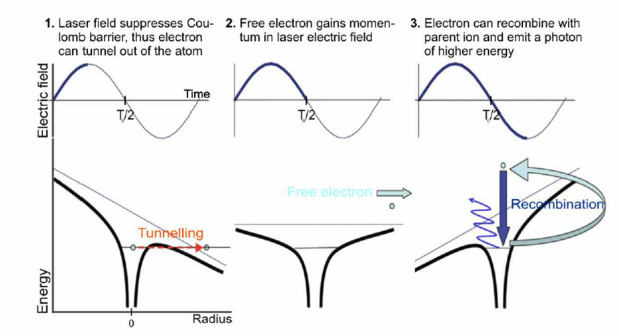
\includegraphics[scale=.30,trim={0 225 0 0}, clip]{images/HHG_Picture1.png}
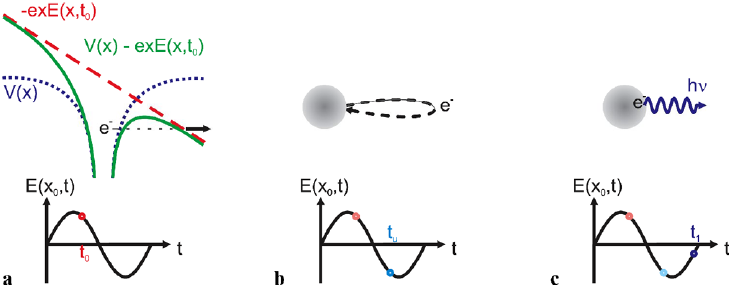
\includegraphics[scale=.2]{images/Classical-three-step-model-14-for-high-harmonics-generation-a-Electron-tunneling.png}
%\footnote{\Tiny Link \textit{et al.}, App. Phys A 96(1):117-135, 2009}
\end{textblock*}

\begin{textblock*}{300pt}(200pt,150pt)
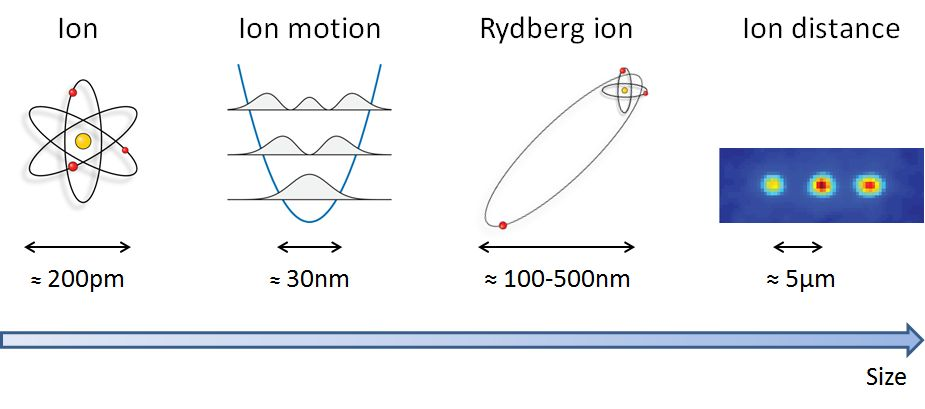
\includegraphics[scale=.15]{images/Dimensions.jpg}
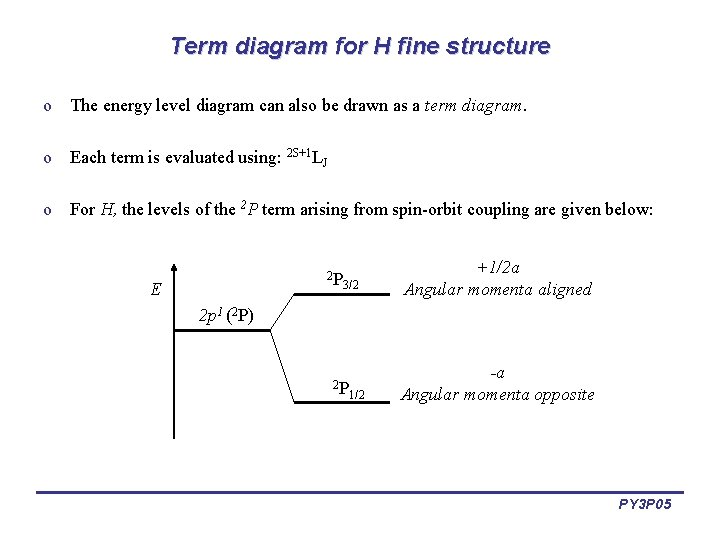
\includegraphics[scale=.25, trim={60 60 320 220},clip]{images/image-6.jpg}
\end{textblock*}


\end{frame}


\begin{frame}
\frametitle{
Role of Spin-Orbit Coupling in High-Order Harmonic Generation
Revealed by Supercycle Rydberg Trajectories
\footnotesize (Phys. Rev. Lett. 129, 173202 (2022))
}
	\framesubtitle{The spin-orbit coupling}
\small
\footnotesize
\begin{textblock*}{400pt}(30pt,60pt)
\begin{itemize}
\item Particles have two different angular momentum which are 
the orbital angular momentum $\boldsymbol{L}$
and spin angular momentum $\boldsymbol{S}.$
\item Their coupling known as the spin-orbit coupling is
\begin{equation}
\left\langle \boldsymbol{L}\cdot\boldsymbol{S} \right\rangle =  
  \frac{\hbar^2}{2}\Big( j(j+1)-\ell(\ell+1) - s(s+1)\Big),
\end{equation}

\noindent induces the shift 
\begin{equation}
\Delta_{SO} =  
  \frac{\beta}{2}\Big( j(j+1)-\ell(\ell+1) - s(s+1)\Big)
\end{equation}

\noindent onto the energy levels $E_n$, who otherwise only depend on
the principal quantum number $n$ and may be degenerated.
\begin{equation}
E_{n\ell} = E_n \pm \Delta_{SO}, \hspace{30pt}
  \beta = \beta(n,\ell) =
     Z^4\frac{\mu_0 }{4\pi}g_s\mu_N^2\frac{1}{n^3a_0^3\ell(\ell+1/2)(\ell+1)}.
\end{equation}
\item Excitation of the spin-orbit split states upon ionization 
can either induces \textit{ultrafast hole dynamics} or entanglement
between the ion and the photoelectron.
\end{itemize}
\end{textblock*}



%\begin{textblock*}{250pt}(40pt,150pt)
%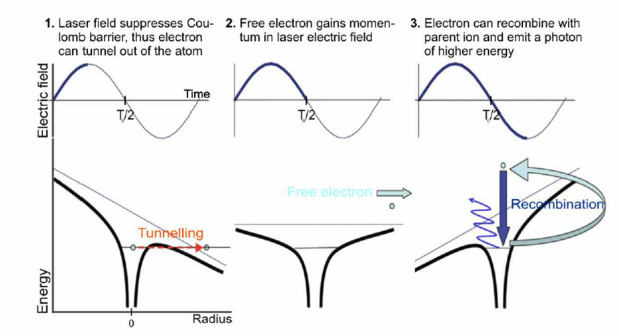
\includegraphics[scale=.30,trim={0 225 0 0}, clip]{images/HHG_Picture1.png}
%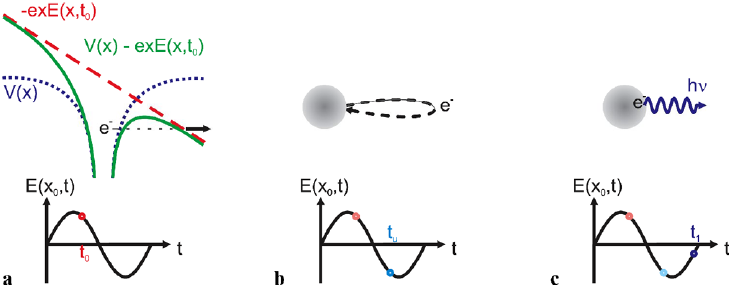
\includegraphics[scale=.2]{images/Classical-three-step-model-14-for-high-harmonics-generation-a-Electron-tunneling.png}\footnote{\Tiny Link \textit{et al.}, App. Phys A 96(1):117-135, 2009}
%\end{textblock*}

\end{frame}




\begin{frame}
\frametitle{
Role of Spin-Orbit Coupling in High-Order Harmonic Generation
Revealed by Supercycle Rydberg Trajectories
\footnotesize (Phys. Rev. Lett. 129, 173202 (2022))
}
	\framesubtitle{The role of the spin-orbit coupling}
\small
\footnotesize
\begin{textblock*}{400pt}(30pt,60pt)
\begin{itemize}
\item Generally thought as negligible because, for Argon, 
the delay $\tau=t_r - t_i \sim 1/\omega$ 
in which you can act upon the hole is too short.
(Because $\tau\Delta_{S0} \ll 1$).
\item Acting upon the hole means dynamically preventing 
an early recombination of the electron in the continnum with the ion
in order to increase the order of the harmonic.
\end{itemize}
\end{textblock*}


\begin{textblock*}{400pt}(30pt,140pt)
\begin{itemize}
\item In this paper, the authors use the \textit{Larmor clock} to identify 
the conbtribution of long-lived Rydberg orbits to the HHG.
\item Moreover, they confirm a results saying that these Rydberg states 
lead to the generation of symmetry forbidden harmonics.
\end{itemize}
\end{textblock*}



%\begin{textblock*}{250pt}(40pt,150pt)
%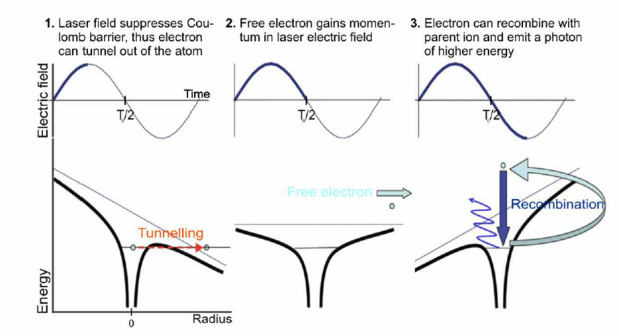
\includegraphics[scale=.30,trim={0 225 0 0}, clip]{images/HHG_Picture1.png}
%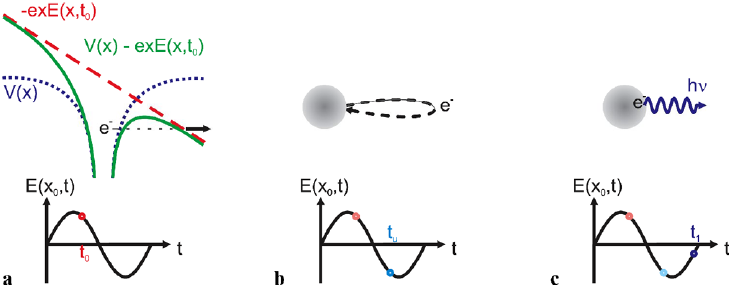
\includegraphics[scale=.2]{images/Classical-three-step-model-14-for-high-harmonics-generation-a-Electron-tunneling.png}\footnote{\Tiny Link \textit{et al.}, App. Phys A 96(1):117-135, 2009}
%\end{textblock*}

\end{frame}


\begin{frame}
\frametitle{
Role of Spin-Orbit Coupling in High-Order Harmonic Generation
Revealed by Supercycle Rydberg Trajectories
\footnotesize (Phys. Rev. Lett. 129, 173202 (2022))
}
	\framesubtitle{The point of these authors}
\small
\footnotesize
\begin{textblock*}{400pt}(30pt,60pt)
\begin{itemize}
\item They use Argon for which for which they can affect 
the precession of the spin  of the hole during the period range 
$T_{SO} = 23.5\, \rm fs$.
\item Note that $T_{SO} $ is the time necessary for the dynamics of the 
spin orbit coupling to take effect and not the period of the laser,
which is $\tau$.
%\footnote{\Tiny which, for a $800\,\rm nm$ laser, is $2.67 \,\rm fs$ by the way.}
\item If and only if $\tau$ spans at least $\tau \sim T_{SO}$, 
the harmonic lines will be split by $\Delta_{SO}$.
\end{itemize}
\end{textblock*}


\begin{textblock*}{400pt}(30pt,140pt)
\begin{itemize}
\item This is what they observe experimentally with a circularly polarized 
$800\,\rm nm$ fundamental field and its second harmonic 
(whose frequency is $2\omega$). 
\item They claim that the fact that they can see those lines is due to those
supercycle trajectories.
\end{itemize}
\end{textblock*}



%\begin{textblock*}{250pt}(40pt,150pt)
%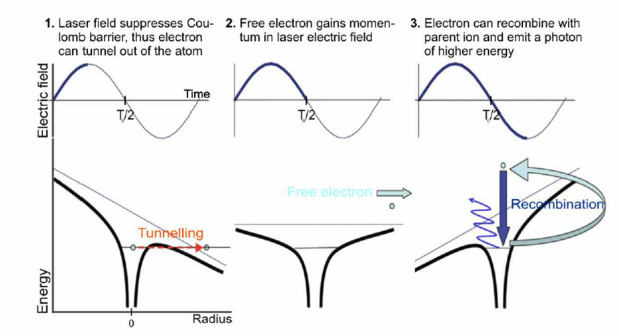
\includegraphics[scale=.30,trim={0 225 0 0}, clip]{images/HHG_Picture1.png}
%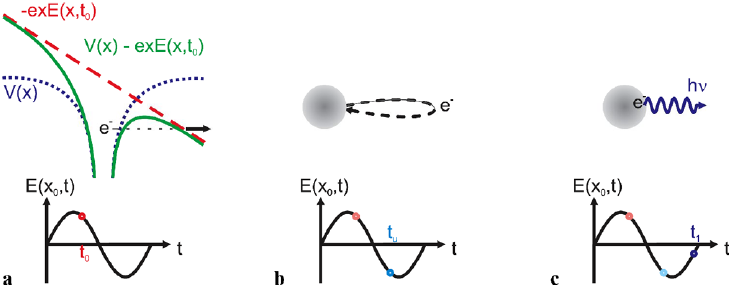
\includegraphics[scale=.2]{images/Classical-three-step-model-14-for-high-harmonics-generation-a-Electron-tunneling.png}\footnote{\Tiny Link \textit{et al.}, App. Phys A 96(1):117-135, 2009}
%\end{textblock*}

\end{frame}



\begin{frame}
\frametitle{
Role of Spin-Orbit Coupling in High-Order Harmonic Generation
Revealed by Supercycle Rydberg Trajectories
\footnotesize (Phys. Rev. Lett. 129, 173202 (2022))
}
	\framesubtitle{Long Rydberg trajectories enhance HHG spectra}
\small
\footnotesize
\begin{textblock*}{190pt}(30pt,60pt)
\begin{itemize}
\item Figure shows the participation of
long-lived Rydberg state to the HHG process.
\item They exist because of Freeman resonances which are the frequency-domain
counterpart to the time-domain frustrated tunneling.
\item Resonance can arise anywhere in the pulse, whenever
\begin{equation}
  E_n + U_p - E_g = n_\omega\omega +  n_{2\omega}2\omega.
\end{equation}
\end{itemize}
\end{textblock*}


\begin{textblock*}{400pt}(30pt,160pt)
\begin{itemize}
\item Resonance emission is liable 
to constructive cycle-to-cycle interference,
when the relative phase 
\begin{equation}
 \phi =  \left(E_n + U_p - E_g\right)T_{\rm cyc} = 2\pi m.
\end{equation}
\item \textbf{Forbidden transition harmonic lines are enabled 
because the ponderomotive energy $U_p$ conserves the 
parity and the angular momentum}.
\end{itemize}
\end{textblock*}



\begin{textblock*}{250pt}(250pt,50pt)
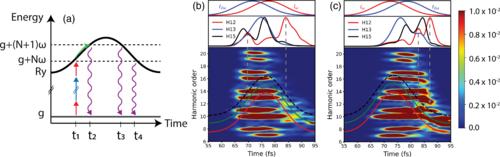
\includegraphics[scale=.7, trim={0 0 310 0}, clip]{images/fig1.png}
\end{textblock*}

\end{frame}


\begin{frame}
\frametitle{
Role of Spin-Orbit Coupling in High-Order Harmonic Generation
Revealed by Supercycle Rydberg Trajectories
\footnotesize (Phys. Rev. Lett. 129, 173202 (2022))
}
	\framesubtitle{Long-lived Rydberg orbits allow parity 
forbidden transitions}
\small
\footnotesize
\begin{textblock*}{190pt}(30pt,60pt)
\begin{itemize}
\item In the case of bicircular $(\omega,2\omega)$,
forbidden harmonics are of order $3N$.
\item Figure shows TDSE calculations in $\rm Ar$,
for two gaussian pulses with FWHM of $15\,\rm fs$ and 
frequency $\omega$ and $2\omega$.
$$
  \omega = 0.057\,\rm a.u.,\hspace{20pt}
  U_p = \sum_{\omega^\prime} U_p^{\omega^\prime} \sim 7\omega.
$$
\end{itemize}
\end{textblock*}


\begin{textblock*}{400pt}(30pt,170pt)
\begin{itemize}
\item The Gabor spectogram shows the two cases where
the $2\omega$ laser precedes the $\omega$ laser (b) 
and vice-versa (b).
\item Ponderomotive shifts of the ground state,
along with the $2p^54s$ and $2p^53d$ states in black, red and green
respectively. 
\item Top panel represents the integration of the Gabor spectrum in 
the $\pm0.25\omega$ range.
\end{itemize}
\end{textblock*}



\begin{textblock*}{250pt}(230pt,70pt)
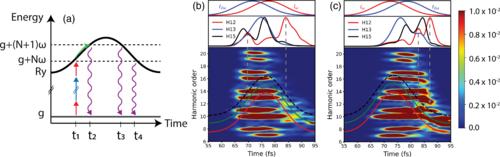
\includegraphics[scale=.55, trim={187 0 0 0}, clip]{images/fig1.png}
\end{textblock*}

\end{frame}


\begin{frame}
\frametitle{
Role of Spin-Orbit Coupling in High-Order Harmonic Generation
Revealed by Supercycle Rydberg Trajectories
\footnotesize (Phys. Rev. Lett. 129, 173202 (2022))
}
	\framesubtitle{Long-lived Rydberg orbits allow the manipulation
of spin-orbit dynamics}
\small
\footnotesize
\begin{textblock*}{190pt}(30pt,60pt)
\begin{itemize}
\item For both $\rm H12$ and $\rm H15$, the contribution of the Rydberg state 
is more visible than for the allowed $\rm H13$.
\item Forbidden lines are made possible by 
the absorption of counterrotating components from either fields.
\end{itemize}
\end{textblock*}


\begin{textblock*}{400pt}(30pt,170pt)
\begin{itemize}
\item When $2\omega$ precedes the fundamental pulse,
enhancement appears in resonance around the peak of the laser.
\item When the fundamental pulse precedes $2\omega$,
enhancement appears around the falling edges.
\item The difference between the two cases when the second harmonic
precedes or follow the fundamental is called 
a \textit{temporal gate}.
\vspace{5pt}
\item \textbf{Rydberg orbits spending a longer time trapped inside the pulse 
allow the resolving of the spin orbit hole dynamics}.
\end{itemize}
\end{textblock*}



\begin{textblock*}{250pt}(230pt,70pt)
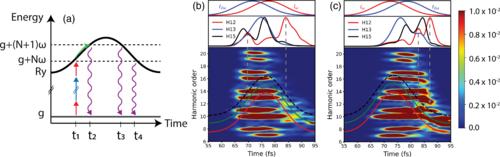
\includegraphics[scale=.55, trim={187 0 0 0}, clip]{images/fig1.png}
\end{textblock*}

\end{frame}


\begin{frame}
\frametitle{
Role of Spin-Orbit Coupling in High-Order Harmonic Generation
Revealed by Supercycle Rydberg Trajectories
\footnotesize (Phys. Rev. Lett. 129, 173202 (2022))
}
	\framesubtitle{The spin-orbit hole dynamics}
\small
\footnotesize
\begin{textblock*}{190pt}(30pt,60pt)
\begin{itemize}
\item Spin orbit temporal modulation of the emission leading to 
spectral splitting of the harmonic lines.
\item The photorecombination amplitude is temporally modulated 
by the factor $1+\exp\left( -i\Delta_{SO}\tau\right)$.
\end{itemize}
\end{textblock*}


\begin{textblock*}{400pt}(30pt,160pt)
\begin{itemize}
\item The point is, they are able to do this experimentally.
\item This is a means to an end to enhance and thus control 
harmonic generation contribution from the Rydberg states.
\item Moreover, they use the spin orbit coupling to 
\begin{itemize}
 \footnotesize
 \item[$\bullet$] experimentally control the precession of the hole 
in the first place, 
 \item[$\bullet$] make sure that what they are seeing
is indeed the effect of the harmonic.
\end{itemize}
\vspace{5pt}
\end{itemize}
\end{textblock*}



\begin{textblock*}{250pt}(250pt,45pt)
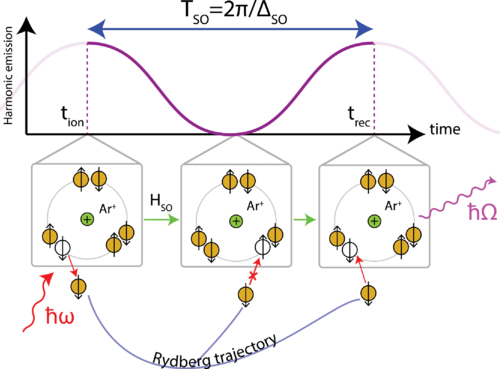
\includegraphics[scale=.33, trim={0 0 0 0}, clip]{images/fig2.png}
\end{textblock*}

\end{frame}


\begin{frame}
\frametitle{
Role of Spin-Orbit Coupling in High-Order Harmonic Generation
Revealed by Supercycle Rydberg Trajectories
\footnotesize (Phys. Rev. Lett. 129, 173202 (2022))
}
	\framesubtitle{Experimental results}
\small
\footnotesize
\begin{textblock*}{250pt}(30pt,60pt)
\begin{itemize}
\item Figure (a) shows the ration between allowed and 
forbidden $3N$ following harmonic line for a $2\omega$ preceding field.
\item The delay dependence of the ratio confirms that symmetry forbidden 
harmonic lines appearing on the falling edge.
\end{itemize}
\end{textblock*}


\begin{textblock*}{250pt}(30pt,120pt)
\begin{itemize}
\item Figure (b) shows "the far field spatially resolved" harmonic spectrum
at positive and negative delays. 
\item At positive delays, strong enhancement of forbidden lines 
can be seen.
\item Furthermore, the spectral splitting of most lines is visible.
\item Absence of the spectral lines for negative time delay
is consistent with discussion.
\vspace{5pt}
\end{itemize}
\end{textblock*}



\begin{textblock*}{250pt}(300pt,45pt)
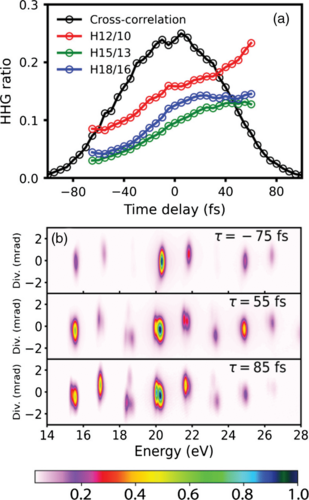
\includegraphics[scale=.4, trim={0 0 0 0}, clip]{images/fig3.png}
\end{textblock*}

\end{frame}


\begin{frame}
\frametitle{
Role of Spin-Orbit Coupling in High-Order Harmonic Generation
Revealed by Supercycle Rydberg Trajectories
\footnotesize (Phys. Rev. Lett. 129, 173202 (2022))
}
	\framesubtitle{Experimental results}
\small
\footnotesize
\begin{textblock*}{250pt}(30pt,60pt)
\begin{itemize}
\item Figure (a) shows role of the spatiotemporal gating
in the generation of harmonics.
\item The Resonance with Stark-shifted Rydberg energies
lead to resonant enhancement for a given harmonic at $x_i$.
\end{itemize}
\end{textblock*}


\begin{textblock*}{250pt}(30pt,120pt)
\begin{itemize}
\item Figure (b) shows "the near-field" profile of $\rm H15$.
\item Upper panel shows the spatial distribution of 
the residual population in the excited state.
Notice that profile looks like panel (a).

\vspace{5pt}
\item Figure (c) shows the spin-orbit splitting of $\rm H15$
in the far-field.
\item Top panel shows frequency-resolved spatially-integrated 
distribution when spin-orbit modulations are included.
\item Right panel shows frequency-integrated spatially-resolved 
$\rm H15$ line.
\end{itemize}
\end{textblock*}



\begin{textblock*}{250pt}(290pt,45pt)
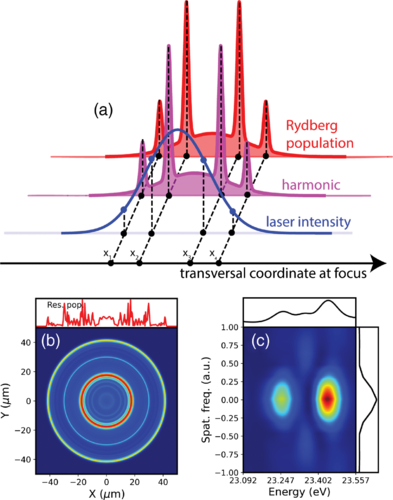
\includegraphics[scale=.4, trim={0 0 0 0}, clip]{images/fig4.png}
\end{textblock*}

\end{frame}


\begin{frame}
\frametitle{
Role of Spin-Orbit Coupling in High-Order Harmonic Generation
Revealed by Supercycle Rydberg Trajectories
\footnotesize (Phys. Rev. Lett. 129, 173202 (2022))
}
	\framesubtitle{Conclusion}
\small
\footnotesize
\begin{textblock*}{400pt}(30pt,60pt)
\begin{itemize}
\item This letter is about the effect of long Rydberg trajectories
onto the HHG spectra for the $\rm Ar$.
\item The harmonic lines are tracked using the spin orbit splitting
and the presence of forbidden lines in the case of counterrotating fundamental
with its second harmonic.
\item This is made possible by the fact that hole dynamics 
can be acted upon in the case of spin-orbit splitting by unlcear means.
\end{itemize}
\end{textblock*}


\begin{textblock*}{400pt}(30pt,150pt)
\begin{itemize}
\item The letter sheds new light on the role of excited states 
in general in the HHG process.
\item Since the timescale can be acted upon through spin-orbit coupling,
experimentalists get to choose between 
\begin{itemize}
\footnotesize
\item[$\bullet$] delayed emission of the pulse train,
\item[$\bullet$] delayed hyper Raman lines in some conditions,
\item[$\bullet$] coherent XUV free-induction decay.
\end{itemize}
\item This is an important step for extending HHG spectroscopy beyond .
the optical cycle 
\end{itemize}
\end{textblock*}




\end{frame}
